%%%%%%%%%%%%%%%%%%%%%%%%%%%%%%%%%%%%%%%%
% datoteka diploma-vzorec.tex
%
% vzorčna datoteka za pisanje diplomskega dela v formatu LaTeX
% na UL Fakulteti za računalništvo in informatiko
%
% vkup spravil Gašper Fijavž, december 2010
% 
%
%
% verzija 12. februar 2014 (besedilo teme, seznam kratic, popravki Gašper Fijavž)
% verzija 10. marec 2014 (redakcijski popravki Zoran Bosnić)
% verzija 11. marec 2014 (redakcijski popravki Gašper Fijavž)
% verzija 15. april 2014 (pdf/a 1b compliance, not really - just claiming, Damjan Cvetan, Gašper Fijavž)
% verzija 23. april 2014 (privzeto cc licenca)
% verzija 16. september 2014 (odmiki strain od roba)
% verzija 28. oktober 2014 (odstranil vpisno številko)
% verija 5. februar 2015 (Literatura v kazalu, online literatura)
% verzija 25. september 2015 (angl. naslov v izjavi o avtorstvu)
% verzija 26. februar 2016 (UL izjava o avtorstvu)
% verzija 16. april 2016 (odstranjena izjava o avtorstvu)
% verzija 5. junij 2016 (Franc Solina dodal vrstice, ki jih je označil s svojim imenom)


\documentclass[a4paper, 12p]{book}
%\documentclass[a4paper, 12pt, draft]{book}  Nalogo preverite tudi z opcijo draft, ki vam bo pokazala, katere vrstice so predolge!

\usepackage[utf8x]{inputenc}   % omogoča uporabo slovenskih črk kodiranih v formatu UTF-8
\usepackage[slovene,english]{babel}    % naloži, med drugim, slovenske delilne vzorce
\usepackage[pdftex]{graphicx}  % omogoča vlaganje slik različnih formatov
\usepackage{fancyhdr}          % poskrbi, na primer, za glave strani
\usepackage{amssymb}           % dodatni simboli
\usepackage{amsmath}           % eqref, npr.
%\usepackage{hyperxmp}
\usepackage[hyphens]{url}  % dodal Solina
\usepackage{comment}       % dodal Solina
\usepackage{listings}

\usepackage[pdftex, colorlinks=true,
						citecolor=black, filecolor=black, 
						linkcolor=black, urlcolor=black,
						pagebackref=false, 
						pdfproducer={LaTeX}, pdfcreator={LaTeX}, hidelinks]{hyperref}
						
\usepackage{pgfplots}

\usepackage{color}       % dodal Solina
\usepackage{soul}       % dodal Solina
\lstdefinelanguage{swift}
{
  morekeywords={
    func,if,then,else,for,in,while,do,switch,case,default,where,break,continue,fallthrough,return,
    typealias,struct,class,enum,protocol,var,func,let,get,set,willSet,didSet,inout,init,deinit,extension,
    subscript,prefix,operator,infix,postfix,precedence,associativity,left,right,none,convenience,dynamic,
    final,lazy,mutating,nonmutating,optional,override,required,static,unowned,safe,weak,internal, integer,
    private,public,is,as,self,unsafe,dynamicType,true,false,nil,Type,Protocol, interface, Int, String, Double, Char, Void, print, type, typ, fun, int, const, NULL, bool, null, Any, abstract, _, def, True, False, putInt
  },
  morecomment=[l]{\#}, % l is for line comment
  morecomment=[s]{/*}{*/}, % s is for start and end delimiter
  morestring=[b]" % defines that strings are enclosed in double quotes
}
\RequirePackage{xcolor}
\definecolor{keyword}{HTML}{BA2CA3}
\definecolor{string}{HTML}{D12F1B}
\definecolor{comment}{HTML}{008400}

\lstset{
  language=swift,
  basicstyle=\ttfamily,
  showstringspaces=false, % lets spaces in strings appear as real spaces
  columns=fixed,
  keepspaces=true,
  keywordstyle=\color{keyword},
  stringstyle=\color{string},
  commentstyle=\color{comment},
  breaklines=true,
  tabsize=2
}

%%%%%%%%%%%%%%%%%%%%%%%%%%%%%%%%%%%%%%%%
%	DIPLOMA INFO
%%%%%%%%%%%%%%%%%%%%%%%%%%%%%%%%%%%%%%%%
\newcommand{\ttitle}{Vgradnja objektno usmerjenih gradnikov v programski jezik PINS}
\newcommand{\ttitleEn}{Diploma thesis sample}
\newcommand{\tsubject}{\ttitle}
\newcommand{\tsubjectEn}{\ttitleEn}
\newcommand{\tauthor}{Toni Kocjan Turk}
\newcommand{\tkeywords}{prevajalnik, programski jezik, sintaksa, semantika, Java, Swift}
\newcommand{\tkeywordsEn}{compiler, programming language, syntax, semantics, Java, Swift}


%%%%%%%%%%%%%%%%%%%%%%%%%%%%%%%%%%%%%%%%
%	HYPERREF SETUP
%%%%%%%%%%%%%%%%%%%%%%%%%%%%%%%%%%%%%%%%
\hypersetup{pdftitle={\ttitle}}
\hypersetup{pdfsubject=\ttitleEn}
\hypersetup{pdfauthor={\tauthor, tk3152@student.uni-lj.si}}
\hypersetup{pdfkeywords=\tkeywordsEn}


 


%%%%%%%%%%%%%%%%%%%%%%%%%%%%%%%%%%%%%%%%
% postavitev strani
%%%%%%%%%%%%%%%%%%%%%%%%%%%%%%%%%%%%%%%%  

\addtolength{\marginparwidth}{-20pt} % robovi za tisk
\addtolength{\oddsidemargin}{40pt}
\addtolength{\evensidemargin}{-40pt}

\renewcommand{\baselinestretch}{1.3} % ustrezen razmik med vrsticami
\setlength{\headheight}{15pt}        % potreben prostor na vrhu
\renewcommand{\chaptermark}[1]%
{\markboth{\MakeUppercase{\thechapter.\ #1}}{}} \renewcommand{\sectionmark}[1]%
{\markright{\MakeUppercase{\thesection.\ #1}}} \renewcommand{\headrulewidth}{0.5pt} \renewcommand{\footrulewidth}{0pt}
\fancyhf{}
\fancyhead[LE,RO]{\sl \thepage} 
%\fancyhead[LO]{\sl \rightmark} \fancyhead[RE]{\sl \leftmark}
\fancyhead[RE]{\sc \tauthor}              % dodal Solina
\fancyhead[LO]{\sc Diplomska naloga}     % dodal Solina


\newcommand{\BibTeX}{{\sc Bib}\TeX}

%%%%%%%%%%%%%%%%%%%%%%%%%%%%%%%%%%%%%%%%
% naslovi
%%%%%%%%%%%%%%%%%%%%%%%%%%%%%%%%%%%%%%%%  


\newcommand{\autfont}{\Large}
\newcommand{\titfont}{\LARGE\bf}
\newcommand{\clearemptydoublepage}{\newpage{\pagestyle{empty}\cleardoublepage}}
\setcounter{tocdepth}{1}	      % globina kazala

%%%%%%%%%%%%%%%%%%%%%%%%%%%%%%%%%%%%%%%%
% konstrukti
%%%%%%%%%%%%%%%%%%%%%%%%%%%%%%%%%%%%%%%%  
\newtheorem{izrek}{Izrek}[chapter]
\newtheorem{trditev}{Trditev}[izrek]
\newenvironment{dokaz}{\emph{Dokaz.}\ }{\hspace{\fill}{$\Box$}}

%%%%%%%%%%%%%%%%%%%%%%%%%%%%%%%%%%%%%%%%%%%%%%%%%%%%%%%%%%%%%%%%%%%%%%%%%%%%%%%
%% PDF-A
%%%%%%%%%%%%%%%%%%%%%%%%%%%%%%%%%%%%%%%%%%%%%%%%%%%%%%%%%%%%%%%%%%%%%%%%%%%%%%%


%%%%%%%%%%%%%%%%%%%%%%%%%%%%%%%%%%%%%%%% 
% define medatata
%%%%%%%%%%%%%%%%%%%%%%%%%%%%%%%%%%%%%%%% 
\def\Title{\ttitle}
\def\Author{\tauthor, tk3152@student.uni-lj.si}
\def\Subject{\ttitleEn}
\def\Keywords{\tkeywordsEn}

%%%%%%%%%%%%%%%%%%%%%%%%%%%%%%%%%%%%%%%% 
% \convertDate converts D:20080419103507+02'00' to 2008-04-19T10:35:07+02:00
%%%%%%%%%%%%%%%%%%%%%%%%%%%%%%%%%%%%%%%% 
\def\convertDate{%
    \getYear
}

{\catcode`\D=12
 \gdef\getYear D:#1#2#3#4{\edef\xYear{#1#2#3#4}\getMonth}
}
\def\getMonth#1#2{\edef\xMonth{#1#2}\getDay}
\def\getDay#1#2{\edef\xDay{#1#2}\getHour}
\def\getHour#1#2{\edef\xHour{#1#2}\getMin}
\def\getMin#1#2{\edef\xMin{#1#2}\getSec}
\def\getSec#1#2{\edef\xSec{#1#2}\getTZh}
\def\getTZh +#1#2{\edef\xTZh{#1#2}\getTZm}
\def\getTZm '#1#2'{%
    \edef\xTZm{#1#2}%
    \edef\convDate{\xYear-\xMonth-\xDay T\xHour:\xMin:\xSec+\xTZh:\xTZm}%
}

\expandafter\convertDate\pdfcreationdate 

%%%%%%%%%%%%%%%%%%%%%%%%%%%%%%%%%%%%%%%%
% get pdftex version string
%%%%%%%%%%%%%%%%%%%%%%%%%%%%%%%%%%%%%%%% 
\newcount\countA
\countA=\pdftexversion
\advance \countA by -100
\def\pdftexVersionStr{pdfTeX-1.\the\countA.\pdftexrevision}


%%%%%%%%%%%%%%%%%%%%%%%%%%%%%%%%%%%%%%%%
% XMP data
%%%%%%%%%%%%%%%%%%%%%%%%%%%%%%%%%%%%%%%%  
\usepackage{xmpincl}
\includexmp{pdfa-1b}

%%%%%%%%%%%%%%%%%%%%%%%%%%%%%%%%%%%%%%%%
% pdfInfo
%%%%%%%%%%%%%%%%%%%%%%%%%%%%%%%%%%%%%%%%  
\pdfinfo{%
    /Title    (\ttitle)
    /Author   (\tauthor, damjan@cvetan.si)
    /Subject  (\ttitleEn)
    /Keywords (\tkeywordsEn)
    /ModDate  (\pdfcreationdate)
    /Trapped  /False
}


%%%%%%%%%%%%%%%%%%%%%%%%%%%%%%%%%%%%%%%%%%%%%%%%%%%%%%%%%%%%%%%%%%%%%%%%%%%%%%%
%%%%%%%%%%%%%%%%%%%%%%%%%%%%%%%%%%%%%%%%%%%%%%%%%%%%%%%%%%%%%%%%%%%%%%%%%%%%%%%

\begin{document}
\selectlanguage{slovene}
\frontmatter
\setcounter{page}{1} %
\renewcommand{\thepage}{}       % preprecimo težave s številkami strani v kazalu
\newcommand{\sn}[1]{"`#1"'}                    % dodal Solina (slovenski narekovaji)

%%%%%%%%%%%%%%%%%%%%%%%%%%%%%%%%%%%%%%%%
%naslovnica
 \thispagestyle{empty}%
   \begin{center}
    {\large\sc Univerza v Ljubljani\\%
      Fakulteta za računalništvo in informatiko}%
    \vskip 10em%
    {\autfont \tauthor\par}%
    {\titfont \ttitle \par}%
    {\vskip 3em \textsc{DIPLOMSKO DELO\\[5mm]         % dodal Solina za ostale študijske programe
	   VISOKOŠOLSKI STROKOVNI ŠTUDIJSKI PROGRAM\\ PRVE STOPNJE\\ RAČUNALNIŠTVO IN INFORMATIKA}\par}%
%    UNIVERZITETNI  ŠTUDIJSKI PROGRAM\\ PRVE STOPNJE\\ RAČUNALNIŠTVO IN INFORMATIKA}\par}%
%    INTERDISCIPLINARNI UNIVERZITETNI\\ ŠTUDIJSKI PROGRAM PRVE STOPNJE\\ RAČUNALNIŠTVO IN MATEMATIKA}\par}%
%    INTERDISCIPLINARNI UNIVERZITETNI\\ ŠTUDIJSKI PROGRAM PRVE STOPNJE\\ UPRAVNA INFORMATIKA}\par}%
%    INTERDISCIPLINARNI UNIVERZITETNI\\ ŠTUDIJSKI PROGRAM PRVE STOPNJE\\ MULTIMEDIJA}\par}%
    \vfill\null%
    {\large \textsc{Mentor}: doc.\ dr.  Bištjan Slivnik\par}%
    {\vskip 2em \large Ljubljana, 2017 \par}%
\end{center}
% prazna stran
%\clearemptydoublepage      % dodal Solina (izjava o licencah itd. se izpiše na hrbtni strani naslovnice)

%%%%%%%%%%%%%%%%%%%%%%%%%%%%%%%%%%%%%%%%
%copyright stran
\thispagestyle{empty}
\vspace*{8cm}

\noindent
{\sc Copyright}. 
Rezultati diplomske naloge so intelektualna lastnina avtorja in Fakultete za računalništvo in informatiko Univerze v Ljubljani.
Za objavo in koriščenje rezultatov diplomske naloge je potrebno pisno privoljenje avtorja, Fakultete za računalništvo in informatiko ter mentorja.

\begin{center}
\mbox{}\vfill
\emph{Besedilo je oblikovano z urejevalnikom besedil \LaTeX.}
\end{center}
% prazna stran
\clearemptydoublepage

%%%%%%%%%%%%%%%%%%%%%%%%%%%%%%%%%%%%%%%%
% stran 3 med uvodnimi listi
\thispagestyle{empty}
\vspace*{4cm}

\noindent
Fakulteta za računalništvo in informatiko izdaja naslednjo nalogo:
\medskip
\begin{tabbing}
\hspace{32mm}\= \hspace{6cm} \= \kill




Tematika naloge:
\end{tabbing}
Besedilo teme diplomskega dela študent prepiše iz študijskega informacijskega sistema, kamor ga je vnesel mentor. V nekaj stavkih bo opisal, kaj pričakuje od kandidatovega diplomskega dela. Kaj so cilji, kakšne metode uporabiti, morda bo zapisal tudi ključno literaturo.
\vspace{15mm}






\vspace{2cm}

% prazna stran
\clearemptydoublepage

% zahvala
\thispagestyle{empty}\mbox{}\vfill\null\it%
\noindent
Na tem mestu zapišite, komu se zahvaljujete za izdelavo diplomske naloge. Pazite, da ne boste koga pozabili. Utegnil vam bo zameriti. Temu se da izogniti tako, da celotno zahvalo izpustite.
\rm\normalfont

% prazna stran
\clearemptydoublepage

%%%%%%%%%%%%%%%%%%%%%%%%%%%%%%%%%%%%%%%%
% posvetilo, če sama zahvala ne zadošča :-)
\thispagestyle{empty}\mbox{}{\vskip0.20\textheight}\mbox{}\hfill\begin{minipage}{0.55\textwidth}%
Svoji dragi Alenčici.
\normalfont\end{minipage}

% prazna stran
\clearemptydoublepage


%%%%%%%%%%%%%%%%%%%%%%%%%%%%%%%%%%%%%%%%
% kazalo
\pagestyle{empty}
\def\thepage{}% preprecimo tezave s stevilkami strani v kazalu
\tableofcontents{}


% prazna stran
\clearemptydoublepage

%%%%%%%%%%%%%%%%%%%%%%%%%%%%%%%%%%%%%%%%
% seznam kratic

\chapter*{Seznam uporabljenih kratic}  % spremenil Solina, da predolge vrstice ne gredo preko desnega roba

\begin{comment}
\begin{tabular}{l|l|l}
  {\bf kratica} & {\bf angleško} & {\bf slovensko} \\ \hline
  % after \\: \hline or \cline{col1-col2} \cline{col3-col4} ...
  {\bf CA} & classification accuracy & klasifikacijska točnost \\
  {\bf DBMS} & database management system & sistem za upravljanje podatkovnih baz \\
  {\bf SVM} & support vector machine & metoda podpornih vektorjev \\
  \dots & \dots & \dots \\
\end{tabular}
\end{comment}

\noindent\begin{tabular}{p{0.1\textwidth}|p{.4\textwidth}|p{.4\textwidth}}    % po potrebi razširi prvo kolono tabele na račun drugih dveh!
  {\bf kratica} & {\bf angleško}                             & {\bf slovensko} \\ \hline
  {\bf CA}      & classification accuracy               & klasifikacijska točnost \\
  {\bf DBMS} & database management system & sistem za upravljanje podatkovnih baz \\
  {\bf SVM}   & support vector machine              & metoda podpornih vektorjev \\
%  \dots & \dots & \dots \\
\end{tabular}


% prazna stran
\clearemptydoublepage

%%%%%%%%%%%%%%%%%%%%%%%%%%%%%%%%%%%%%%%%
% povzetek
\addcontentsline{toc}{chapter}{Povzetek}
\chapter*{Povzetek}

\noindent\textbf{Naslov:} \ttitle
\bigskip

\noindent\textbf{Avtor:} \tauthor
\bigskip

%\noindent\textbf{Povzetek:} 
V diplomskem delu bom predstavil programski jezik Atheris, ki je nastal kot nadgradnja programskega jezika PINS. Prog. jezik PINS, oz. prevajalnik zanj, je bil zgrajen tekom semestra pri predmetu prevajalniki in navidezni stroji. Ker mi je bilo delo na prevajalniku izjemno zanimivo, sem se odločil, da ustvarim svoj programski jezik in sam določim pravila zanj.\\
\indent V diplomskem delu na kratko predstavim prevajalnike in programske jezike, kaj sploh so in kaj je njihov namen. Opišem kakšne so sodobne prakse pri ravoju prevajalnikov, s kakšnimi probleme se prevajalnik sooča ter kako je zgrajen. \\
\indent Podrobneje bom obrazložil nadgradnje jezika PINS, s kakšnimi problemi sem se tekom razvoja soočal ter kako sem jih reševal. Pokazal bom nekaj primerov programov v mojem jeziku ter primerjal z drugimi jeziki.

\noindent 

\bigskip

\noindent\textbf{Ključne besede:} \tkeywords.
% prazna stran
\clearemptydoublepage

%%%%%%%%%%%%%%%%%%%%%%%%%%%%%%%%%%%%%%%%
% abstract
\selectlanguage{english}
\addcontentsline{toc}{chapter}{Abstract}
\chapter*{Abstract}

\noindent\textbf{Title:} \ttitleEn
\bigskip

\noindent\textbf{Author:} \tauthor
\bigskip

%\noindent\textbf{Abstract:} 
\noindent This sample document presents an approach to typesetting your BSc thesis using \LaTeX. 
A proper abstract should contain around 100 words which makes this one way too short.
\bigskip

\noindent\textbf{Keywords:} \tkeywordsEn.
\selectlanguage{slovene}
% prazna stran
\clearemptydoublepage

%%%%%%%%%%%%%%%%%%%%%%%%%%%%%%%%%%%%%%%%
\mainmatter
\setcounter{page}{1}
\pagestyle{fancy}

\chapter{Uvod}

Razvoj prevajalnikov, ter s tem tudi programskih jezikov, je, po mojem mnenju, izjemno pomembna panoga v računalništvu. Programski jezik je medij, preko katerega komuniciramo z računalnikom. Prevajalniki razvijalcem omogočajo, da se med razvojem programske opreme ne rabijo osredotočati na nizkovojske detajle, ampak se lahko posvetijo reševanju praktičnih problemov. Naloga prevajalnika je, da pretvori človeku berljivo kodo v računalniku razumljivo zaporedje strojnih ukazov. \\
\indent Dandanes lahko za razvoj programske opreme izbiramo med veliko programskih jezikov. Trenutno eni izmed najbolj popularnih so JavaScript, Java, Python in C++, popularnost pa dobivajo tudi novejši jeziki, kot so GoLang, Swift, Kotlin in podobni. [1] \\
\indent S prevajalniki sem se začel ukvarjati pri predmetu Prevajalniki in Navidezni Stroji (PINS) v drugem letnik na Fakulteti za Računalništvo in Informatiko. Tekom diplomske naloge bom predstavil programski jezik Atheris ter prevajalnik zanj. Osredotočil se bom predvsem na vgradnjo objektno usmerjenih gradnikov v programski jezik.

\chapter{Prevajalniki}
\label{ch0}

\section{Uvod v prevajalnike in programske jezike}

Programski jezik je poseben jezik, ki se uporabljaja za razvoj programske opreme. Programski sistemi, ki poskrbijo, da se izvede pretvorba kode, napisane v programskem jeziku, v računalniku razumljivo obliko, se imenujejo \textit{prevajalniki}. \\
Nekaj definicij:
\begin{enumerate}  
	\item \textbf{Računski model (angl. computational model):} zbirka vrednosti in računskih operacij 
	\item \textbf{Izračun (angl. computation)}: zaporodje operacij nad vrednostjo (ali več vrednosti), ki vrne nek rezultat
	\item \textbf{Program:} specifikacija izračuna
	\item \textbf{Programski jezik:} zapis (notacija) za pisanje programov
\end{enumerate}
\cite{computationalModel}

Program lahko predstavimo kot funkcijo, pri kateri je rezultat (angl. \textit{output}) funkcija vhodnih parametrov (angl. \textit{input}):
\begin{lstlisting}
	rezultat = program(vhodni parametri)
\end{lstlisting}

Iz drugega zornega kota si lahko program predstavljamo tudi kot model problemske domene, kjer je instanca izvedbe programa simulacija problema:
\begin{lstlisting}
	program = model problemske domene
	izvedba programa = simulacija problema
\end{lstlisting}
\cite{computationalModel}

\section{Zgradba prevajalnika}

Sodobni prevajalniki so pogosto organizirani v več posameznih faz, vsaka izmed njih pa operira na različnem nivoju abstrakcije jezika. \cite{modernCompiler}

\begin{figure}[h]
	\begin{center}
		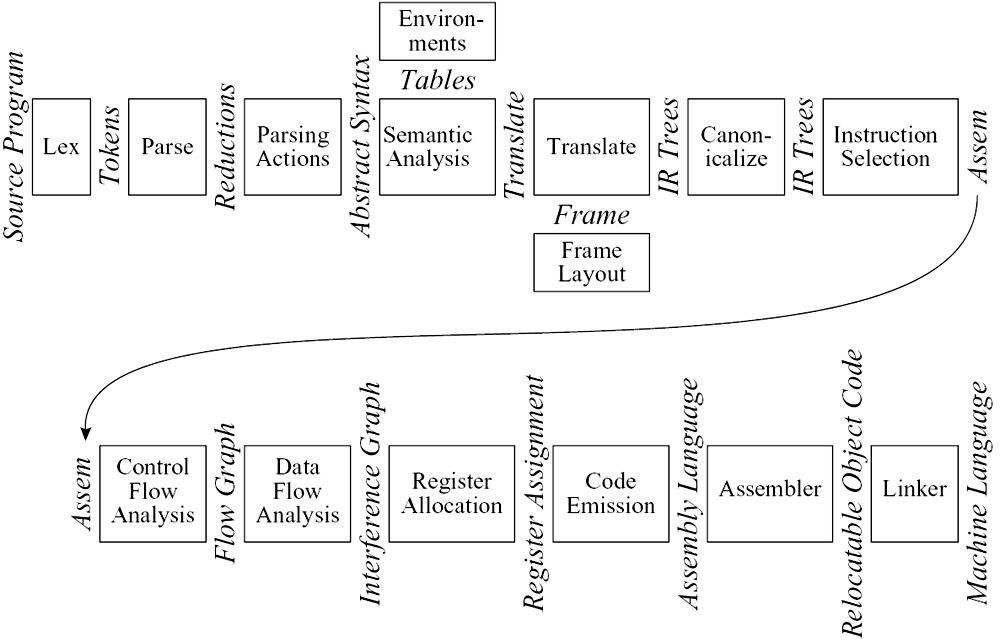
\includegraphics[width=1\textwidth]{resources/compilerPhases.jpg}
	\end{center}
	\caption{Faze prevajalnika ter vmesniki, ki jih povezujejo med seboj.}
	\label{pic1}
\end{figure}

Zato da lahko prevajalnik program prevede iz ene oblike v drugo, ga mora najprej analizirati, razumeti njegovo strukturo ter pomen, šele nato ga pretvori nazaj v drugačno obliko.  \\
Analizo programa običajno delimo v naslednje korake:
\begin{enumerate}
	\item \textbf{Leksikalna analiza} (angl. \textit{lexical analysis})
	\item \textbf{Sintaksna analiza} (angl. \textit{syntax analysis})
	\item \textbf{Semantična analiza} (angl. \textit{semantic analysis})
\end{enumerate}
\cite{modernCompiler}

\subsection{Leksikalna analiza}

Tako imenovani leksikalni analizator kot vhod prejme tok znakov (angl. \textit{stream of characters}), kot izhod pa vrne tok v naprej definiranih žetonov (angl. \textit{stream of tokens}). Žeton je običajno zgrajen iz imena, vrednosti (t.i. \textit{lexeme}) ter lokacije v izvorni datoteki.  \cite{modernCompiler}

\subsubsection{Leksikalni žetoni:}

Žeton (ali simbol) je zaporedje znakov, ki ga interpretiramo kot samostojno enoto v slovnici programskega jezika. \cite{modernCompiler}\\ 
Tabela \ref{tabel:vrsteZetonov} prikazuje nekaj vrst simbolov ter primere.\\

\begin{table}
	\begin{center}
		\begin{tabular}{l|c|c}
			\textbf{vrsta žetona} & \textbf{angl.} & \textbf{primeri} \\ \hline\hline
			ime & identifier & x	foo		bar		thisIsAnIdentifier \\
			rezervirana beseda & keyword & while	for		if		public	override \\
			operator & operator & , 	. 		\&\& 	=		== \\
			niz znakov & string & "this is a string" \\
			znak & character & 'a' 		'x' 	'@' \\
			celo št. & integer & 10 	125 	082 \\
			decimalno št. & real & 201.5 	3.14	1.2e10
		\end{tabular}
	\end{center}
	\caption{Primeri žetonov v programskem jeziku Java}
	\label{tabel:vrsteZetonov}
\end{table}

\newpage

\begin{lstlisting}[caption={Primer programa v programskem jeziku Atheris},label={lst:atherisCode}, captionpos=b]
	let x: Int
	let y: Int
	x * y
\end{lstlisting}
Rezultat:
\begin{lstlisting}[caption={Rezultat leksikalne analize za program ~\ref{lst:atherisCode}},captionpos=b]
	[1:1-1:4] 	LET:let
	[1:5-1:6] 	IDENTIFIER:x
	[1:6-1:7] 	COLON::
	[1:8-1:11] 	IDENTIFIER:Int
	[1:11-1:12] 	NEWLINE:\n
	[2:1-2:4] 	LET:let
	[2:5-2:6] 	IDENTIFIER:y
	[2:6-2:7] 	COLON::
	[2:8-2:11] 	IDENTIFIER:Int
	[2:11-2:12] 	NEWLINE:\n
	[3:1-3:2] 	IDENTIFIER:x
	[3:3-3:4] 	MUL:*
	[3:5-3:6] 	IDENTIFIER:y
	EOF:$
\end{lstlisting}

\subsection{Sintaksna analiza}

Druga faza prevajanja je sintaksna analiza (angl. \textit{syntax analysis} ali \textit{parsing}). Naloga te faze je, da zagotovi, da je napisan program slovnično pravilen in v skladu s sintaksnimi pravili. Sintaksni analizator prejme kot vhod tok žetonov, ki ga zgenerira prejšnja faza, rezultat pa je abstraktno sintaksno drevo.\\
\indent\textbf{Abstraktno sintaksno drevo} (AST) je drevesna podatkovna struktura, ki predstavlja slovnično strukturo programa. Vsako vozlišče drevesa ponazarja konstrukt v programski kodi.\\

\begin{figure}[h]
	\begin{center}
		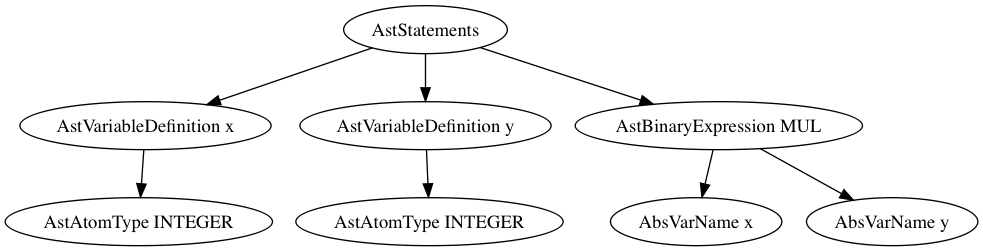
\includegraphics[width=1\textwidth]{resources/ast.png}
	\end{center}
	\caption{Abstraktno sintaksno drevo za program ~\ref{lst:atherisCode}.}
	\label{image:ast}
\end{figure}

Iz slike ~\ref{image:ast} lahko razberemo, da gre za dve definiciji spremenljivk in množenje.\\
\indent Abstraktno sintaksno drevo je bistvenega pomena, saj nadaljne faze operirajo izključno nad njim.

\subsection{Semantična analiza}

Semantična analiza poveže definicije spremenljivk z njihovimi uporabami ter preveri, ali so vsi izrazi pravilnih podatkovnih tipov. \cite{modernCompiler}\\
\indent Običajno semantično analizo razdelimo na dve pod-fazi:
\begin{enumerate}
	\item \textbf{Razreševanje imen:} zagotovi, da za vsako uporabo imena obstaja znotraj trenutnega območja vidnosti definicija z istim imenom, ter uporabo poveže z definicijo
	\item \textbf{Preverjanje tipov:} vsakemu vozlišču v AST določi podatkovni tip, ter na podlagi postavljenih semantičnih pravil zagotovi, da so vsi izrazi pravilnih tipov
\end{enumerate}

\begin{figure}[h]
	\begin{center}
		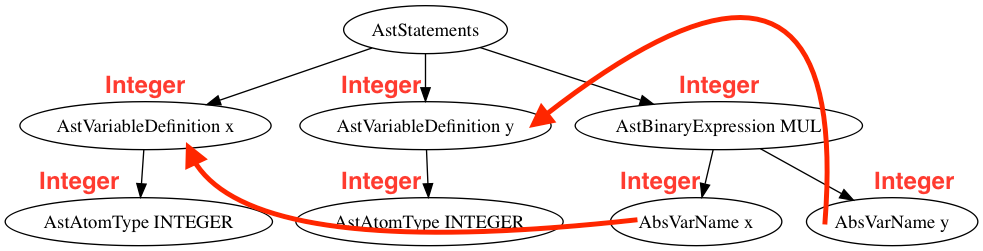
\includegraphics[width=1\textwidth]{resources/astSeman.png}
	\end{center}
	\caption{Rezultat semantične analize za program ~\ref{lst:atherisCode}}
	\label{image:astSeman}
\end{figure}

Pri implementaciji semantične analize nam pomaga \textit{simbolna tabela}.

\subsubsection{Simbolna tabela}

Simbolna tabela je podatkovna struktura, ki mapira imena v njihove definicije in podatkovne tipe. \cite{modernCompiler} Ker običajno programi vsebujejo več tisoč unikatnih definicij imen, mora podatkovna struktura omogočati učinkovito poizvedovanje. Iz slike ~\ref{image:astSeman} lahko razberemo, kaj se med izvajanjem semantične analize zgodi v ozadju: puščice predstavljajo povezave med definicijami in uporabami, evaluacija podatkovnih tipov pa je pri vseh vozliščih \textit{Integer}, razen pri korenu, ki nima tipa oz. je tipa \textit{Void}.\\
\indent Kot sem omenil, semantična analiza zagotovi, da za vsako uporabo imena obstaja njena definicija, in da so podatkovni tipi pravilni. Sledita dva primera, kjer to ne drži:

\begin{lstlisting}[caption={Primer programa, kjer spremenljivka \textit{y} ni definirana},label={lst:atherisCodeNameError},captionpos=b]
	let x: Int
	print(y)
\end{lstlisting}

\begin{figure}[h]
	\begin{center}
		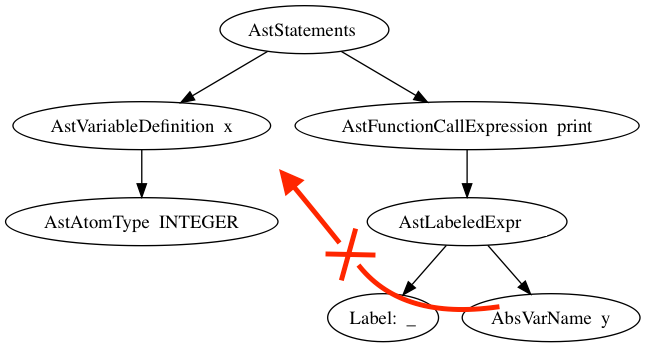
\includegraphics[width=0.9\textwidth]{resources/astSemanNameError.png}
	\end{center}
	\caption{Napaka v programu ~\ref{lst:atherisCodeNameError}. Spremenljivka \textit{y} ni definirana.}
	\label{image:astSemanCodeNameError}
\end{figure}

\begin{lstlisting}[caption={Primer programa, kjer je napaka v podatkovnih tipih},label={lst:atherisCodeTypeError},captionpos=b]
	let x: Int
	let s: String
	x + s
\end{lstlisting}

\begin{figure}[h]
	\begin{center}
		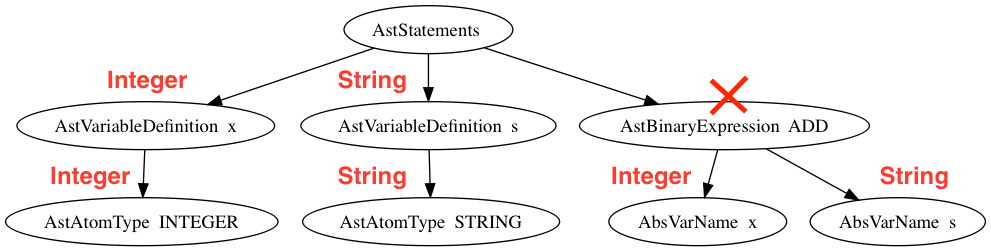
\includegraphics[width=0.9\textwidth]{resources/astSemanTypeError.png}
	\end{center}
	\caption{Napaka v programu ~\ref{lst:atherisCodeTypeError}. Seštevanje med podatkovnima tipoma \textit{Integer} in \textit{String} ni dovoljeno.}
	\label{image:astSemanTypeError}
\end{figure}

\subsection{Klicni zapisi}

V skoraj vsakem modernem programskem jeziku ima lahko funkcija \textit{lokalne} spremenljivke, ki so kreirane ob vstopu v funkcijo. Hkrati lahko naenkrat obstaja več zapisov iste funkcije, zato je pomembno, da ima vsak zapis lastne instance lokalnih spremenljivk. \cite{modernCompiler} \\
\indent V funkciji 
\begin{lstlisting}
todo
\end{lstlisting}

se za vsak njen klic ustvari nova instanca x, ki jo inicializira klicalec funkcije. Ker je funkcija rekurzivna, živi v pomnilniku naenkrat veliko x-ev. Podobno se ob vsakem vstopu v jedro funkcije ustvari tudi nova instanca y. \cite{modernCompiler}\\

\subsubsection{Sklad}

Klicni zapisi funkcij se shranjujejo na sklad. Sklad je v pomnilniku predstavljen kot velika tabela s posebnim registrom imenovanim \textit{stack pointer}, ki kaže na konec sklada. Ob vsakem klicu funkcije se sklad poveča za velikost klicnega zapisa klicane funkcije. Podobno se ob vrnitvi funkcije zmanjša za enako vrednost. Prostor v klicnem zapisu namenjen hrambi vhodnih parametrov, lokalnih spremenljivk in ostalih registrov se imenuje \textit{activation record}. \cite{modernCompiler}
\\\\
\textbf{Kazalec na klicni zapis}

Predpostavimo da funkcija \textit{g} kliče funkcijo \textit{f}. Ob vstopu v f kazalec na sklad (SP) kaže na prvi vhodni argument funkciji f. Nov prostor na skladu je rezerviran tako, da se od SP odšteje velikost klicnega zapisa f. Tako SP sedaj kaže na konec sklada. Stara vrednost SP postane nova vrednost kazalca na klicni zapis (\textit{angl. frame pointer}). V programskih jezikih, kjer je velikost klicnega zapisa za posamezno funkcijo konstantna, je vrednost kazalca na klicni (FP) zapis vedno izračunljiva, zato si je ni potrebno posebaj shranjevati na sklad. FP = SP + velikost sklada. \cite{modernCompiler}

\textbf{Prenos parametrov}

Standarden način klicanja funkcij je, da klicoča funkcija rezervira prostor na skladu za prenosih njenih izhodnih parametrov (oz. vhodnih parametrov za klicano funkcijo). \cite{modernCompiler} \\
\indent Prostor za njih se običajno nahaja pred SP. Klicana funkcija tako naslov njenega i-tega parametra izračuna z enačbo 
\begin{lstlisting}
	argumentAddress(i) = FP + (4 * i)
\end{lstlisting}

\textbf{Lokalne spremenljivke}

Prevajalnik mora na skladu alocirati dovolj prostora za vse lokalne spremenljivke. todo

\textbf{Static link}

V jezikih, ki podpirajo gnezdenje funkcij, lahko gnezdene funkcije dostopajo do spremenljivk, ki se nahajajo v zunanjih funkcijah. Da lahko gnezdena funkcija dostopa do spremenljivk, ki niso na njenem klicnem zapisu, ji ob klicu poleg ostalih parametrov posredujemo FP funkcije, ki jo neposredno definira. Temu kazalcu rečemo \textit{static link}. 

\begin{lstlisting}[caption={Primer gnezdenih funkcij}, captionpos=b, label={lst:nestedFunctions}]
    func f() {
        var x: Int = 10
        func e() {
            var z: Int = 100
        }
        func g() {
            var y: Int = 20
            func h() {
                print(y, x)
            }
        }
    }
\end{lstlisting}

Primer ~\ref{lst:nestedFunctions} vsebuje dve gnezdeni funkciji \textit{g} in \textit{h}. Funkcija h lahko dostopa do spremenljivk definiranih v \textit{g} in \textit{f}, ne pa tudi tistih v \textit{e}.

\subsection{Generiranje vmesne kode}   

\subsubsection{Vmesna koda}

Vmesna koda (\textit{angl. intermidiate representation}) je abstraktna predstavitev strojnega jezika in predstavlja ukaze, brez da bi poznali arhitekturo ciljne naprave. Poleg tega je vmesna koda neodvisna od izvornega jezika. \cite{modernCompiler} \\
\indent Dobra predstavitev vmesne kode ima naslednje lastnosti:

\begin{enumerate}
	\item Njegovo generiranje mora biti priročno
	\item Generiranje strojne kode v dejansko strojno kodo mora biti priročno za vse ciljne arhitekture
	\item Vsak gradnik mora imeti jasen pomen, da so lahko optimizacijske transformacije enostavno implementirane
\end{enumerate}
\cite{modernCompiler}

Posamezni deli abstraktnega sintaksnega drevesa so lahko kompleksne stvari, na primer zanke, klici funkcij, itd., ki jih ne moremo neposredno mapirati v strojne ukaze. Zato morajo gradniki vmesne kode predstavljati le enostavne operacije, kot so npr. LOAD (preberi vrednost iz pomnilnika), STORE (shrani vrednost v pomnilnik), ADD (seštej dve vrednosti), itd. Tako lahko vsak posamezen del AST prevedemo v ravno pravo zsaporedje ukazov abstraktne vmesne kode. \cite{modernCompiler} \\ 

\chapter{Programski jezik PINS}

Programski jezik PINS je učni programski jezik, zato je tudi dokaj preprost. Prevajalnik zanj smo implementiral v sklopu domačih nalog pri predmetu Prevajalniki in navidezni stroji.

\section{Leksikalna pravila}

Programski jezik PINS podpira tri atomarne podatkovne tipe: \textit{integer}, \textit{logical}, \textit{string}, za katere so rezervirane istoimenske besede. Celoštevilske konstante so poljubno predznačeno zaporedje števk, logične konstante so ali \textit{true} ali \textit{false}, znakovne konstante pa so definirane kot poljubno (lahko prazno) zaporedje znakov z ASCII kodami med vključno 32 in 126, ki je obdano z enojnima navednicama (ASCII koda 39); izjema je en sam enojni narekovaj, ki je podvojen. \\
\indent Imena so definirana kot poljubno zaporedje črtk, številk in podčrtajev, ki se ne začne s številko in ni rezervirana beseda ali kakšna od prej naštetih konstant. \\
\indent Belo besedilo (\textit{angl. whitespace}) so presledki (ASCII 32), tabulatorji (ASCII 9) in znaka za konec vrstice (ASCII 10 in 13). \\
\indent Komentarji se začnejo z '\#' (ASCII 35) in se raztezajo do konca vrstice.

\section{Sintaksna pravila}

Celotna izvorna koda je sestavljena iz seznama definicij. Vsaka definicija je lahko:

\begin{enumerate}
	\item Definicija tipa (oz. sklic na tip - \textit{typealias})
	\item Definicija spremenljivke
	\item Definicija funkcije
\end{enumerate}

Kot sem že omenil, podpira PINS tri osnovne podatkovne tipe, vendar sintaksa omogoča tudi definicijo tabel (\textit{angl. array}) s fiksno velikostjo. \\
\indent Definicija funkcije je sestavljena iz imena, seznama parametrov, tipa ki ga funkcija vrača, ter \textit{izraza} oz. jedra funkcije. Zanimivo pri PINSu je to, da izven jedra funkcij ne moremo početi ničesar drugega, kot ustvarjati definicije (podobno kot pri Javi). \\
\indent Izraz (\textit{angl. expression}) je lahko:
\begin{enumerate}
	\item Logični izraz
	\item Primerjalni izraz
	\item Seštevalni izraz
	\item Multiplikativni izraz
	\item Seštevalni izraz
	\item Prefiksni izraz
	\item Postfiksni izraz
	\item Atomarni izraz
\end{enumerate}

Atomarni izraz se še naprej deli in je lahko:
\begin{enumerate}
	\item Logična konstanta
	\item Celoštevilska konstanta
	\item Znakovna konstanta
	\item Ime
	\item Klic funkcije
	\item If stavek
	\item If else stavek
	\item While stavek
	\item Zaporedje izrazov
\end{enumerate}

Vsakemu izrazu lahko sledijo tudi definicije gnezdene znotraj zavitih oklepajev.

\section{Semantična pravila}

\subsubsection{Območja vidnosti}

Imena so vidna v celotnem območju vidnosti, ne glede na mesto definicije. Izraz \textit{expression \{ WHERE definitions \}} ustvari novo vgnezdeno območje vidnosti. To pomeni, da definicije znotraj zavitih oklepajev niso vidne navzven. Tudi definicija funkcije ustvari novo vgnezdeno območje vidnosti, ki se začne za imenom in se razteza do konca funkcije..

\subsubsection{Tipiziranost}

\begin{enumerate}
	\item \textit{integer}, \textit{logical}, \textit{string} opisujejo podatkovne tipe INTEGER, LOGICAL in STRING, zaporedoma
	\item izraz 
\begin{lstlisting}[]
	arr [ n ] type
\end{lstlisting}
	opisuje podatkovni tip ARR(n, type), kjer je \textit{n} celoštevilska konstanta 
\end{enumerate}

\subsubsection{Deklaracije}

\begin{enumerate}
	\item Deklaracija tipa
\[
typ\quad  identifier\quad  :\quad  type
\]
	ustvari sklic na podatkovni tip \textit{type} z imenom \textit{identifier}
	\item Deklaracija funkcije
%\begin{lstlisting}[]
\[ fun\quad identifier  ( identifier_1 : type_1, ..., identifier_n : type_n ) : type = expression \]
%\end{lstlisting}
	določa funkcijo, ki je tipa \[type_1 \quad *, \quad  ..., \quad *\quad  type_n \,\to\, type \]
	\item Deklaracija spremenljivke
\[
var \quad identifier\quad :\quad type
\]

določa spremeljivko tipa $type$
	\item Deklaracija parametra
\[
identifier \quad :\quad type
\]
določa parameter tipa $type$
\end{enumerate}

\chapter{Programski jezik Atheris}
\label{ch1}

Kljub temu, da prevajalnik za Atheris izhaja iz prevajalnika za PINS, sta si jezika med seboj zelo različna. Razlikujeta se predvsem v sintaksi, ki je v programskem jeziku Atheris zelo podobna tisti, ki jo ima programski jezik Swift. \\
\begin{figure}[h]
	\begin{center}
		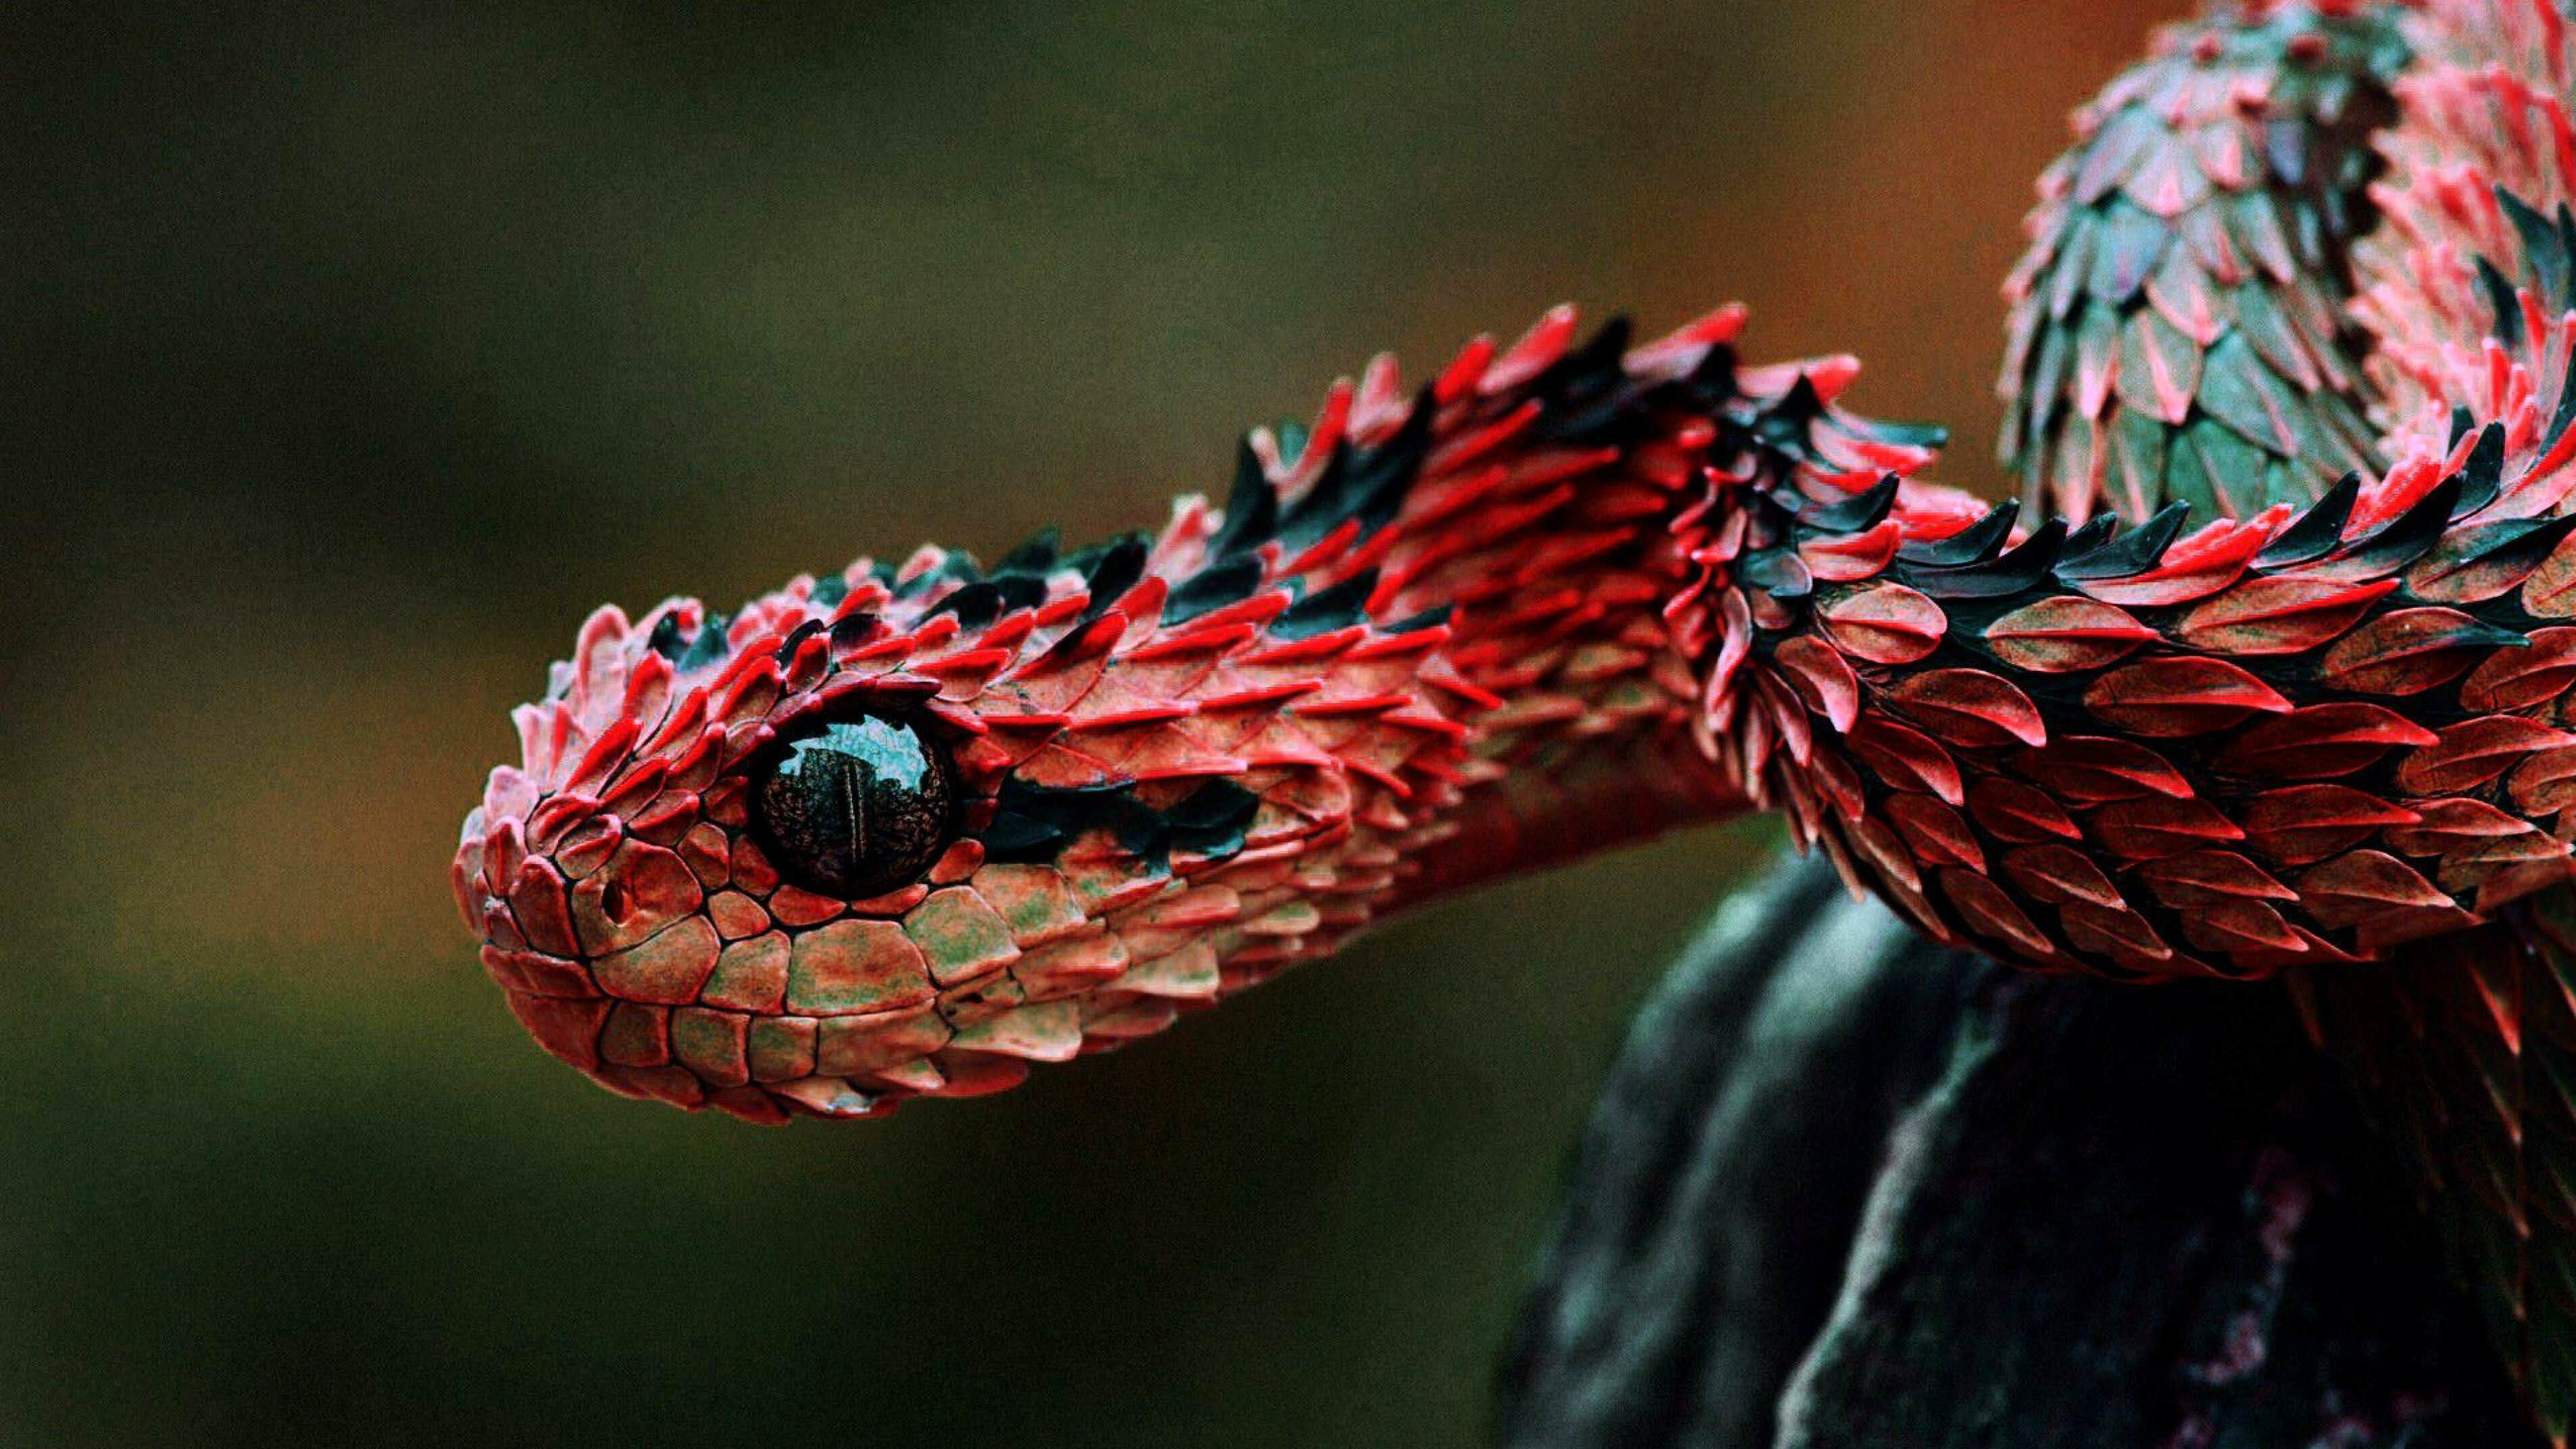
\includegraphics[width=1\textwidth]{resources/atheris.jpg}
	\end{center}
	\caption{Atheris Squamigera. [http://rebrn.com/]}
	\label{image:ast}
\end{figure}

\indent Med drugim nova sintaksa omogoča definiranje kompleksnejših podatkovnih tipov z uporabo razredov, vmesnikov, terk in enumeracij. \\
\indent Posamezni stavki so med seboj ločeni z novimi vrsticami (Python, Swift), vendar pa prevajalnik omogoča njihovo ločevanje tudi s podpičjem ';' (C++, Java). \\
\indent Komentarji se lahko začnejo bodisi z '\#' in se raztezajo do konca vrstice (Python, PINS), bodisi z '/*' in končajo z '*/' (Java, C++). \\
\indent Podprt je tudi \textit{switch} kontrolni stavek s sintakso identične tej od Swifta.\\
\indent Definicije funkcij ter klici funkcij so spremenjeni; parametri funkcije so sedaj sestavljeni iz labele ter imena parametra (tako kot v Swiftu). Pri klicu funkcije se uprabi labela parametra, znotraj jedra funkcije pa se uporablja ime.

\subsection{Podatkovni tipi}

Podprti atomarni podatkovni tipi so: \textit{integer, double, string, char} in \textit{bool}. Poleg atomarnih tipov pa so podprti tudi sestavljeni podatkovni tipi:

\begin{enumerate}
	\item Razredi
	\item Enumeracije
	\item Terke
\end{enumerate}

Poleg naštetih podatkovnih tipov obstaja še podatkovni tip, ki ga ni mogoče eksplicitno uporabljati. To je kazalec (\textit{angl. pointer}). Ena izmed prednosti kazalcev je v tem, da lahko do kompleksnejših objektov, ki v pomnilniku zasedejo veliko prostora, dostopamo preko njihovega naslova s kazalcem, namesto kopiranja celotne vsebine (na primer pri pošiljanju objekta kot argument funkciji). Spremeljivke, ki jim priredimo objekt, terko ali tabelo, se implicitno smatrajo kot kazalci. \\

\section{Sintaksa}

Celoten program v jeziku PINS je sestavljen iz seznama definicij, definicija pa je lahko definicija spremenljivke, definicija tipa ali definicija funkcije. Sintaksa programskega jezika Atheris se razlikuje v tem, da je program sestavljen iz zaporedja stavkov, stavek pa je lahko \textit{izraz} ali \textit{definicija}. Definicije so predstavljene z naslednjimi konteksno neodvisnimi gramatikami:

\begin{enumerate}
	\item Spremenljivke
\begin{lstlisting}[]
var_def -> visibility var identifier 
var_def -> visibility var identifier = expression
var_def -> visibility var identifier: type 
var_def -> visibility var identifier: type = expression 

visibility -> public
visibility -> private
visibility -> $
\end{lstlisting}
	\item Funkcije
\begin{lstlisting}[]
func_def -> func identifier ( parameters ) { statements }
func_def -> func identifier ( parameters ) 
type { statements }

parameters -> $
parameters -> paramater
parameters -> paramaters, paramater

parameter -> identifier : type
parameter -> identifier identifier : type
\end{lstlisting}	
	\item Enumeracije
	
\begin{lstlisting}
enum_def -> enum { enum_defs }

enum_defs -> $
enum_defs -> enum_member_def
enum_defs -> enum_defs, enum_member_def

enum_member_def -> case identifier
enum_member_def -> case identifier = expression (literal)
enum_member_def -> enum_member_def, enum_member_def // todo
\end{lstlisting}
	\item Terke
\begin{lstlisting}
todo
\end{lstlisting}
	\item Razredi
\begin{lstlisting}
class_def -> class { definitions }
\end{lstlisting}

\end{enumerate} 

Sintaksa izrazov je skoraj identična PINSu, razen izrazov za nadzor toka (angl. \textit{control flow}):

\begin{enumerate}
	\item If stavek
\begin{lstlisting}[]
if_expression { statements } if_expression'
if_expression' -> $
if_expression' -> else if { statements } if_expression'
if_expression' -> else { statements }
\end{lstlisting}
	\item Switch stavek
\begin{lstlisting}[]
switch_expression { cases }

cases -> case expressions : statements cases'
cases' -> $
cases' -> cases
cases' -> default : statements
\end{lstlisting}
	\item While stavek
\begin{lstlisting}[]
while_expression -> while expression { statements }
\end{lstlisting}
	\item For stavek
\begin{lstlisting}[]
for_expression -> for identifier in expression 
{ statements }
\end{lstlisting}
\end{enumerate} 

Kot sem že omenil, omogoča sintaksa programskega jezika Atheris, da so posamezni stavki ločeni bodisi s ';' bodisi z novo vrstico. Za ta namen je dodan nov tip žetona, ki predstavlja novo vrstico v izvorni kodi (pred tem se je znak za novo vrstico štel kot belo besedilo). V primeru, da je v izvorni kodi več zaporednih novih vrstic, jih leksikalni analizator \textit{požre} in vedno vrne samo en zaporedni \textit{newline} simbol. To naredi sintaksno analizo enostavnejšo. 

\section{Funkcije}

Programski jezik Atheris zahteva, da ob klicu funkcij poleg imena funkcije navedemo tudi imena parametrov. Podobno kot to zahteva tudi Swift. \\
\indent Ob deklaraciji funkcije lahko opcijsko definiramo poljubno število poimenovanih ter tipiziranih vrednosti, ki jim skupaj rečemo parametri funkcije. Poleg tega lahko opcijsko navedemo še podatkovni tip vrednosti, ki jo bo funkcija vračala (privzeto funkcije ne vračajo ničesar - \textit{Void}.) \\
\indent Imena parametrov so sestavljena iz dveh delov: labele argumenta ter imena parametra. Labele argumentov se uporabljajo ob klicu funkcije, medtem ko se imena parametrov uporabljajo znotraj jedra funkcije. Labele so privzeto identične imenom.

\begin{lstlisting}[caption={Primer definicije in klica funkcije}, captionpos=b]
func someFunction(firstParameterName: Int, secondParameterName: Int) {
  /* znotraj telesa funkcije, sta firstParameterName in secondParameterName referenci na vrednosti argumentov za prvi in drugi parameter. */
}
someFunction(firstParameterName: 1, secondParameterName: 2)
\end{lstlisting}

\subsection{Določanje label argumentov}

Če želimo, da sta labela in ime različna, navedemo labelo argumenta pred imenom:

\begin{lstlisting}[caption={Labela argumenta in ime parametra se razlikujeta}, captionpos=b]
func someFunction(argumentLabel parameterName: Int) {
/* znotraj telesa funkcije, se parameterName sklicuje na vrednost argumentza funkciji */
}
someFunction(argumentLabel: 1) 
\end{lstlisting}

Podprta je tudi možnost, da se izognemo navajanju imen argumentov pri klicanju funkcij. To storimo tako, da označimo labelo argumenta z '\_'.

\begin{lstlisting}[caption={}, captionpos=b]
func someFunction(_ firstParameterName: Int, _ secondParameterName: Int) {
  ///
}
someFunction(1, 2)
\end{lstlisting}

V ozadju so opisane funkcionalnosti implementirane tako, da se v simbolno tabelo ne shrani samo \textit{ime} funkcije, ampak se celotna definicija pretvori v posebno znakovno predstavitev, ki je sestavljena iz imena ter label argumentov. Funkcije z istim imenom, a različnimi imeni parametrov, lahko tako shranimo v simbolno tabelo brez težav. Znakovne predstavitve zgornjih funkcij izgledajo tako:

\begin{lstlisting}[caption={Znakovne predstavitve funkcij}, captionpos=b]
someFunction(firstParameterName:secondParameterName)
someFunction(argumentLabel)
someFunction(_:_)
\end{lstlisting}

T.i. \textit{overloadanje} funkcij sedaj ni problem, saj čeprav imajo funkcije ista imena, vsako izmed njih predstavimo z drugim imenom, zato jih lahko v simbolni tabeli ustrezno poiščemo. Seveda je potrebno v podobni obliki predstaviti tudi klice funkcij.


\section{Enumeracije}

V primeru, da enumeracija nima surovih vrednosti, je semantična analiza dokaj preprosta. Kompleksnejša postane kadar so surove vrednosti prisotne, saj je potrebno zagotoviti, da so ustreznega podatkovnega tipa. V primeru, da surove vrednosti niso eksplicitno navedene, jih prevajalnik skuša določiti sam. To lahko stori samo v primeru, če so surove vrednosti tipa \textbf{Int} ali \textbf{String}. \\
\indent Privzeto so surove vrednosti za \textbf{Int} zaporedna števila začenši z 0. V primeru, da je vrednost eksplicitno navedena, je vrednost naslednje surove vrednosti naslednje zaporedno število od prejšnje vrednosti.

\begin{lstlisting}[caption={Enumeracija s surovimi vrednostmi tipa Int}, captionpos=b]
	enum Days: Int {
	  case Monday // vrednost = 0
	  case Tuesday = 10 // vrednost = 10
	  case Wednesday // vrednost = 11
	  case Thursday = 100 // vrednost = 100
	  case Friday // vrednost = 101
	}
\end{lstlisting}

\indent Za \textbf{String} so privzete surove vrednosti imena članov enumeracije.

\begin{lstlisting}[caption={Enumeracija s surovimi vrednostmi tipa String}, captionpos=b, label={lst:fruitEnumeration}]
	enum Fruit: String {
	  case Apple // privzeta vrednost = "Apple"
	  case Orange = "Annoying Orange"
	  case Strawberry // privzeta vrednost = "Strawberry"
	}
\end{lstlisting}

Do posameznih elementov enumeracije dostopamo z \textit{DOT} operatorjem ('.'), kjer je na levi strani ime enumeracije, na desni pa ime elementa. Podobno dostopamo tudi do surovih vrednosti z uporabo imena \textit{rawValue}. Operator DOT bom podrobneje opisal na razdelku razredov, za zdaj lahko povem da je njegova naloga to, da zagotovi, da v sestavljenem podaktovnem tipu na levi strani obstaja član z imenom na desni strani.

\begin{lstlisting}[caption={Primer dostopa do elementov enumeracije ~\ref{lst:fruitEnumeration}}, captionpos=b]
	print(Fruit.Apple.rawValue) // 'Apple'
	print(Fruit.Orange.rawValue)  // 'Annoying Orange'
	print(Fruit.Strawberry.rawValue)  // 'Strawberry'
\end{lstlisting}

Člane enumeracije lahko prirejamo spremenljivkam ter nad njimi izvajamo logični operaciji primerjanja vrednosti. 

\begin{lstlisting}[caption={}, captionpos=b]
	let x: Languages = Languages.Cpp
	if x == Languages.Java {
	    print("Java")
	}
	else {
	    print("Some other language")
	}
\end{lstlisting}

Da lahko realiziramo \textit{runtime} operacije nad člani enumeracije, prevajalnik vsak član enumeracije nadomesti z njegovim indeksom v definiciji enumeracije. Za zgornji primer bo tako spremeljivka \textit{x} vsebovala vrednost 0. V \textit{if} stavku primerjamo vrednosti 0 in 1, iz česar sledi, da se bo izvedel \textit{else} blok.

\newpage
\section{Terke}

Terka je podatkovna struktura sestavljena iz poljubnega števila elementov, ki so lahko različnih podatkovnih tipov. Terke poznajo jeziki, kot sta Python in Swift, medtem ko jih Java in C++ ne poznata.\\
\indent Terka je definirana kot zaporedje izrazov znotraj oklepajev. Do posameznih elementov terke dostopamo podobno kot dostopamo do elementov v razredu, s to razliko, da je ime elementa njegov indeks v terki. Vsakemu izrazu znotraj terke lahko opcijsko določimo tudi ime. V primeru, da ime ni eksplicitno določeno, se za ime uporabi indeks izraza v terki (začenši z 0). \\
\indent Do elementov prav tako dostopamo z uporabo DOT operatorja, ki zagotovi, da terka vsebuje izraz z željenim imenom.\\
\indent V pomnilniku so terke predstavljene skoraj identično kot tabele, s to razliko, da se podatkovni tipi elementov med sabo lahko razlikujejo. Ravno zaradi tega ne moremo odmika izračunati na enak način kot pri tabelah. Pri terkah odmik posameznega elementa od začetnega naslova terke izračunamo tako, da seštejemo velikosti podaktovnih tipov vseh elementov pred željenim elementom:

\[ offset ( element_i )  = sum ( size ( element_0 ), size( element_1 ), ..., size ( element_n-1)) \]

\section{Razredi}

Razred je sestavljena podatkovna struktura, ki, podobno kot terka, v sebi hrani spremenljivke različnih podatkovnih tipov. Vsak razred lahko vsebuje poljubno število atributov (spremenljivk) ter poljubno število metod - to so člani rezreda. \\
\indent Atributi in metode so lahko statični, kar pomeni, da niso del posamezne instance razreda, ampak živijo v statični instanci, ki je kreirana avtomatsko. Poleg tega so lahko člani razreda \textit{privatni} ali \textit{javni}. Razlika je v tem, da do privatnih članov ni možno dostopati izven razreda.\\
\indent Metodam lahko dodamo tudi modifikator \textit{final}, kar prepreči, da bi bila funkcija re-implementirana v dedujočem se razredu. Če želimo, da metoda re-implementira metodo v starševkem razredu, ji moramo dodati modifikator \textit{overriding}. \\
\indent Poleg atributov in metod lahko razred vsebuje tudi definicije gnezdenih razredov, enumeracij ter vmesnikov.\\
\indent V pomnilniku je instanca razreda (objekt) predstavljena podobno kot terka, t.j. kot tabela z vrednostmi različnih podatkovnih tipov. Zato tudi odmik elementov izračunamo podobno kot pri terkah.

\subsection{Dostop do članov in nadzor dostopa}

Do članov razreda dostopamo preko DOT operatorja. DOT operator je binarni operator in je sestavljen iz dveh izrazov, ki ju povezuje pika '.'. \\
\indent Običajno se izvaja povezovanje uporab spremenljivk z definicijami v fazi razreševanja imen, vendar to pri sestavljenih podatkovnih strukturah (vključno z enumeracijami in terkami) ni mogoče.\\
\indent Zato se s tem ne ukvarjamo v razreševanju imen, ampak problem prepustimo razreševanju tipov. Razreševanje tipov zato delimo na dve pod-fazi (dva sprehoda po AST). V prvem sprehodu nas zanimajo samo podatkovni tipi definicij, izraze zaenkrat pustimo pri miru. Ko zberemo vse potrebne informacije o podatkovnih tipih članov razreda, lahko zgradimo razredni tip, ki predstavlja razred in njegove definicije. \\
\indent Sedaj imamo dovolj informacij, da razrešimo imena znotraj DOT operatorja, kar storimo v drugem sprehodu.\\

\textbf{Nadzor dostopa}

Nadzor dostopa omejuje dostop do članov razreda izven definicije, če to eksplicitno navedemo z uporabo modifikatorja \textit{\textbf{private}}. Privzeto so vsi člani \textit{\textbf{public}}. Programski jezik Atheris trenutno pozna samo public in private modifikatorja; public modifikator omogoča dostop do in spreminjanje vrednosti člana razreda kodi, ki se ne nahaja v razredu, za razliko od modifikatorja private, ko to prepoveduje. 

\subsection{Instančne funkcije}

Razred ima lahko v sebi definirane funkcije, ki se jim v OOP žargonu pogosto reče \textit{metode}. Metode se od funkcij, ki niso definirane v razredu, razlikuje v tem, da vsebujejo impliciten parameter, ki je referenca na objekt, ki metodo kliče. Ta parameter prevajalnik v metodo vstavi avtomatsko. \\
\indent V C++ in Javi se ta parameter imenuje \textbf{\textit{this}}, v Pythonu, Swiftu in v Atherisu pa \textbf{\textit{self}}. V Pythonu je ta razlika, da je parameter potrebno eksplicitno navesti, če ga ne, se funkcija / metoda smatra kot statična (več o statičnih metodah v nadaljevanju). \\
\indent Prevajalnik mora implicitni \textit{self} parameter avtomatsko vstaviti v vse metode razreda. Delno to stori tekom razreševanja imen, ko definiciji funkcije vstavi nov parameter, delno pa tekom razreševanja tipov, ko parametru nastavi tip razreda. \\

\subsection{Konstruktorji}

Konstruktorji so posebne vrste metod, njihova naloga pa je kreacija objektov ter inicializacija atributov. Podobno kot ostalim metodam razreda tudi konstruktorju prevajalnik implicitno vstavi \textit{self} parameter. \\
\indent Naloga konstruktorja je, da na kopici, t.j. delu pomnilnika, kamor shranjujemo dinamično alicirane objekte (za razliko od sklada, kamor shranjujemo statične), alocira prostor, kjer bo shranjen objekt. Za dinamično alociranje pomnilnika se uporabi gradnik vmesne kode \textbf{ImcMALLOC}. Ta gradnik na kopici rezervira željeno velikost pomnilnika ter vrne naslov. \\
\indent Pri generiranju vmesne kode prevajalnik vstavi na začetek kode funkcije MALLOC gradnik, ki bo rezerviral prostor za objekt. Nato bo prevajalnik vrnjen naslov shranil na sklad v parameter \textit{self}, zato da lahko znotraj konstruktorja nastavimo vrednosti ostalih atributov razreda. Na koncu bo ta naslov konstruktor tudi vrnil. Vrnjen naslov je referenca na objekt in ga uporabljamo za nadaljne operacije nad objektom. \\
\indent Razred ima lahko poljubno število konstruktorjev, ki jih definiramo z uporabo ključne besede \textit{\textbf{init}}. 
\newpage

\begin{lstlisting}[caption={Konsturktorji}, captionpos=b]
	class Atheris {
	    var x: Int
	    init() {
	        self.x = 0
	    }
	    init(x: Int) {
	        self.x = x
	    }
	}
\end{lstlisting}

\indent Poleg eksplicitnih konstruktorjev prevajalnik zgenerira tudi impliciten \textit{privzeti} konstruktor. Vanj je vstavljena koda za inicializacijo atributov, ki so inicializirani ob definiciji. 

\begin{lstlisting}[caption={Implicitni privzeti konstruktor}, captionpos=b]
	class Atheris {
	    var x: Int = 10
	    var y: Int = 20
	}
	
	print(Atheris().x) // 10
	print(Atheris().y) // 20
\end{lstlisting}

V primeru, da je v razredu privzeti konstruktor tudi eksplicitno definiran, bo poleg svoje kode vseboval tudi kodo implicitnega.

\begin{lstlisting}[caption={Eksplicitni privzeti konstruktor}, captionpos=b]
	class Atheris {
	    var x: Int = 10
	    var y: Int = 20
	    init() { // privzeti konstruktor
	        y = 100
	    }
	}
	
	print(Atheris().x) // 10
	print(Atheris().y) // 100
\end{lstlisting}

\subsection{Statični člani razreda}

Statični člani razreda so tisti člani, ki ne živijo znotraj posameznih instanc, ampak živijo v globalni statični instanci razreda. Definiramo jih z uporabo modifikatorja \textit{\textbf{static}}. Statična instanca razreda je naložena v pomnilnik avtomatsko ob zagonu programa. Do statičnih članov dostopamo preko imena razreda. Ker statične funkcije niso del instance razreda, ne vsebujejo \textit{self} parametra.

\begin{lstlisting}[caption={Klicanje statične funkcije}, captionpos=b]
	class Static {
   	    static func foo() {
	         print("I am a static function")
	    }
	} 
	Static.foo()
\end{lstlisting}

\indent V času razreševanja tipov so statične definicije razreda shranjene v ločeno podatkovno strukturo od instančnih. Vozlišču AST, ki definira razred (\textit{AstClassDefinition}), v simbolno tabelo ne pripišemo razredni podatkovni tip, ampak \textit{statični / kanonični} tip, ki hrani podatke o statičnih definicijah razreda ter referenco na dejanski instačni podatkovni tip. Ko se sklicujemo na člane statične instance preko DOT operatorja, prevajalnik preveri, ali statični tip vsebuje iskan član.\\
\indent Razredi lahko vsebujejo tudi enumeracije in gnezdene razrede. Definicije enumeracij in razredov se smatrajo privzeto kot statične, zato do njih dostopamo enako kot do statičnih članov. 

\begin{lstlisting}[caption={Enumeracija znotraj razreda}, captionpos=b]
	class Static {
	    enum Languages: Int {
	        case Cpp, Java
	    }
	}
	let x = Static.Languages.Java
	print(x.rawValue) // '1'
\end{lstlisting}

Da lahko dostopamo do konstruktorjev znotraj gnezdenih razredov, jih prevajalnik smatra, kot da so to statične metode.

\begin{lstlisting}[caption={Gnezden razred}, captionpos=b]
	class Atheris {
	    class NestedClass {
	        var x = 20
	    }
	}
	print(Atheris.NestedClass().x) // '20'
\end{lstlisting}

\section{Dedovanje in polimorfizem}

Dedovanje in polimorfizem sta, poleg enkapsulacije in abstrakcije, najpomembnejša koncepta OOP programiranja. Dedovanje je mehanizem, s katerim objekt pridobi (podeduje) nakatere ali vse lastnosti drugega objekta, medtem ko je polimorfizem sposobnost predstaviti isto funkcionalnost z različnimi implementacijami. Programski jezik Atheris omogoča enkratno dedovanje, tako kot Java in Swift. \\
\indent V pomnilniku se atributi dedovanega razreda nahajajo pred atributi dedujočega se razreda. Enačba za izračun velikosti razreda (koliko prostora porabi objekt v pomnilniku) postane kompleksnejša, saj je potrebno rekurzivno prišteti velikosti nadrazradov. Prav tako postane komleksnejši izračun odmikov atributov od začetnega naslova. 

\subsection{Dynamic Dispatch} \label{dynamicDispatch}

Dynamic dispatch je proces izbire, katera implementacija polimorfne operacije naj se izvede v času \textbf{izvajanja programa}. Običajno lahko pri klicih funkcij že v času prevajanja izberemo, katera \textit{implementacija} funkcije naj se kliče, saj obstaja samo ena. Pri razredih nastane problem, kadar dovolimo, da imajo lahko dedujoči se razredi svoje implementacije funkcij (oz. metod), kot je razvidno v spodnjem primeru: 

\begin{lstlisting}[caption={Več implementacij za isto funkcionalnost}, captionpos=b]
	class Fruit {
	    func kind() {
	        print("I am a Fruit!")
	    }
	}
	class Apple: Fruit {
	    override func kind() {
	        print("I am an Apple!")
	    }
	}
	class Orange: Fruit {
	    override func kind() {
	        print("I am an Orange!")
	    }
	}
\end{lstlisting}

\indent Problem je možno rešiti na več načinov. Rešitev prevajalnika za Atheris temelji na rešitvi, ki jo ima tipično C++, t.j. z uporabo podatkovne strukture \textit{\textbf{v-table}}. 

\subsubsection{Virtualna tabela}

Virtualna tabela je podatkovna stuktura, ki vsebuje kazalce na funkcije implementirane v danem razredu. Prevajalnik za vsak razred zgenerira in shrani v pomnilnik unikatno virtualno tabelo. \\
\indent Vsak objekt v pomnilniku, poleg svojih atributov, hrani še kazalec na lastno virtualno tabelo.

\begin{figure}[h]
	\begin{center}
		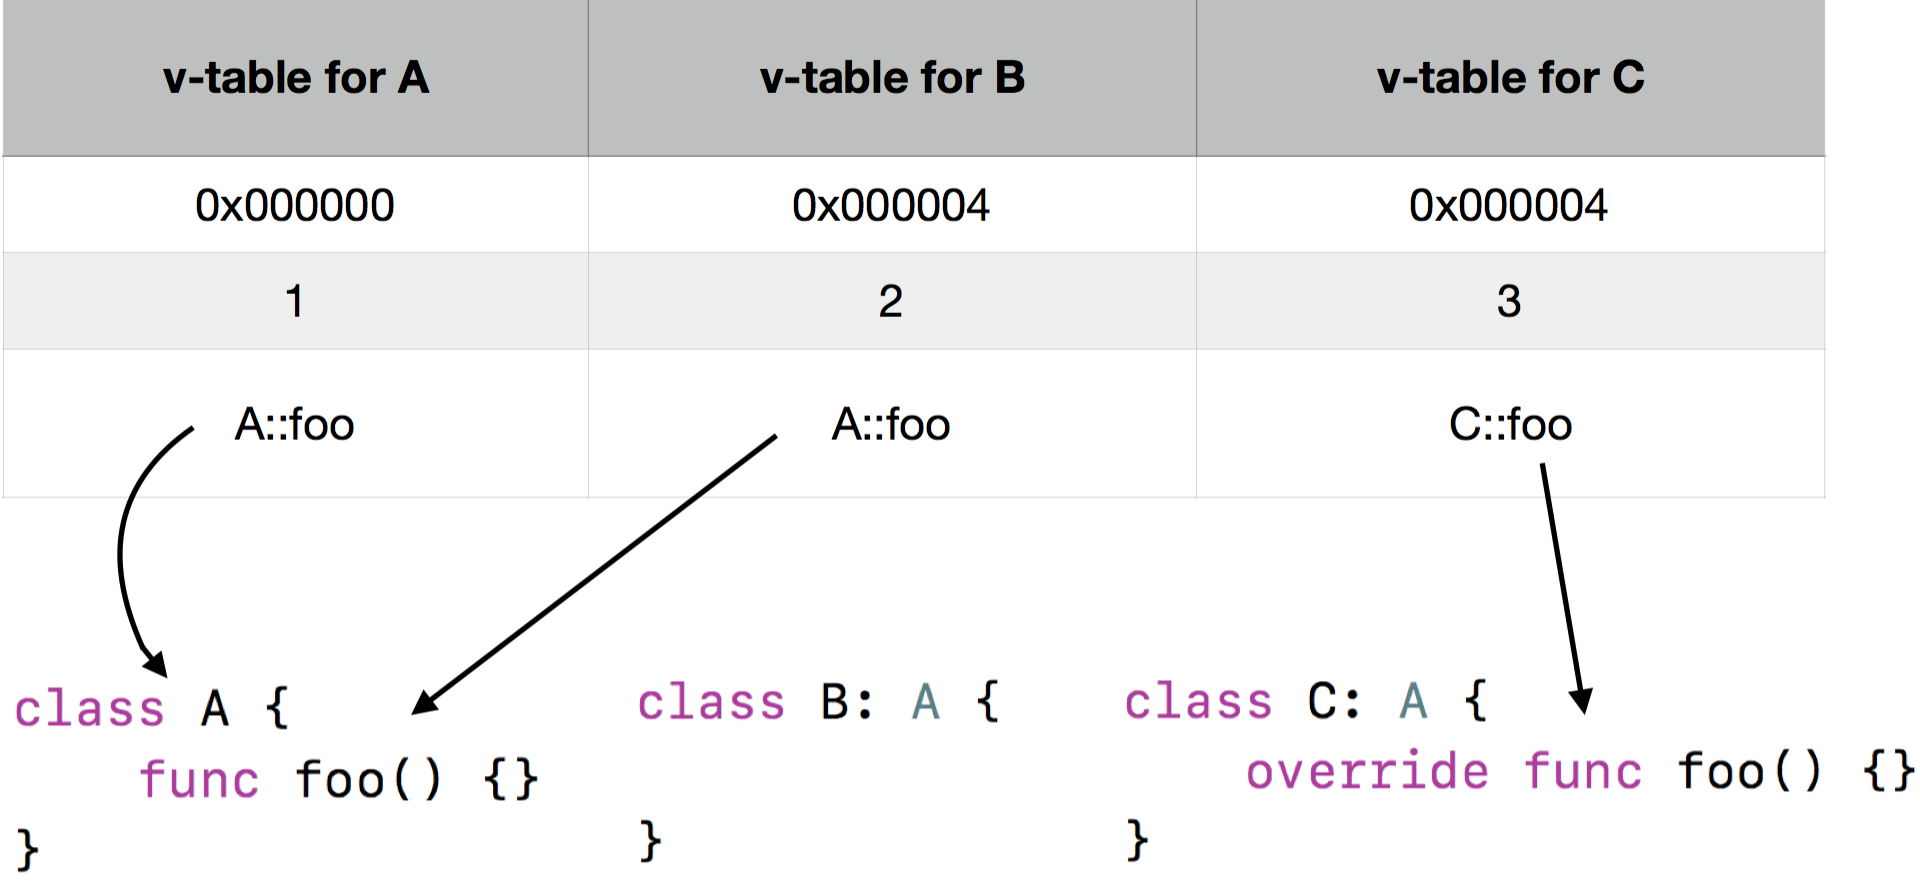
\includegraphics[width=1\textwidth]{resources/v-tables.png}
	\end{center}
	\caption{Virtualne tabele za dane razrede. (todo popravi shemo da uporabiš razrede iz zgornjega primera)}
	\label{vtables}
\end{figure}

Virtualna tabela vsebuje kazalce na naslove, kjer se nahajajo vse ne-statične metode, ki so implementirane v razredu. Vsaka tabela vsebuje še kazalec na virtualno tabelo nadrazreda (ali \textit{null}, če ga nima), ter unikatni identifikator tipa. Identifikator je pozitivno celo število, ki ga prevajalnik dodeli vsakemu tipu in je unikaten za vsak tip. \\

\subsection{Realizacija}

Problem rešimo tako, da kazalec na metodo shranimo v virtualno tabelo na tisti indeks, na katerem je motoda definirana v razredu. Prevajalnik za klic funkcije zgenerira vmesno kodo, ki izračuna naslov metode z naslednjo enačbo:

\[ address(method_i) = adress(vtable) + (i * sizeof(void*) + 8) \]

kjer je \[address(vtable)\]\ lokacija tabele v pomnilniku, \[(i * sizeof(void*) + 8)\] indeks pomnožen z velikostjo kazalca (običajno 4 byti) plus odmik od začetka tabele zaradi prej opisanih dodatnih podatkov v tabeli in \[ address(method_i)\] naslov metode na indeksu i.

\section{Instance of operator}

Instance of operator je operator, ki v času izvajanja programa preveri, ali je objekt instanca danega razreda. To naredi z uporabo virtualne tabele. Kot sem omenil, vsaka tabela vsebuje unikatni deskriptor njenega razreda. Preko deskriptorja lahko preverimo, ali se dva podatkovna tipa ujemata. \\
\indent V programskem jeziku Atheris se operator imenuje \textit{is}.

\begin{lstlisting}[caption={Uporaba operatorja \textit{is} za razrede iz sheme ~\ref{vtables}}, captionpos=b]
	var object: A
	object = B()
	print(object is A) // 'true'
	print(object is B) // 'true'
	print(object is C) // 'false'
\end{lstlisting}

Dejanski algoritem za preverjanje, ali je objekt instanca danega razreda, je  kompleksnejši kot sem opisal zgoraj, saj je lahko razredna hiearhija obsežna in je zato potrebno preverjanje izvesti rekurzivno po celotni hiearhiji.

\begin{lstlisting}[caption={Algoritem za izračun ali je objekt instanca danega razeda}, captionpos=b]
todo
\end{lstlisting}

\newpage

\section{Pretvarjanje tipov}

Mehanizem pretvarjanja iz enega tipa v drug (angl. \textit{type casting}) deluje po zelo podobnem principu kot \textit{as} operator. Razlikujeta se predvsem v njunem rezultatu. Rezultat \textit{as} operatorja je \textit{true} ali \textit{false}, medtem ko je pri neuspešnem pretvarjanju rezultat \textit{null}, pri uspešnem pa objekt, pretvorjen v željen tip. Takemu tipu pretvarjanja rečemo \textit{safe casting}, saj program nadaljuje z izvajanjem tudi če pretvorba ni uspešna. Za razliko od \textit{non-safe castanja}, kjer bi program vrnil \textit{null pointer exception}.

\begin{lstlisting}[caption={Pretvorba za razrede iz sheme ~\ref{vtables}}, captionpos=b]
	var object: A = B()
	let casted = object as B
	    print("cast failed")
	}
	else {
	    print("cast succeeded") // izvede se 'else' blok
	}
\end{lstlisting}

\section{Vmesniki}

Vmesnik je abstraken opis akcij, ki jih lahko izvede objekt. Tekom prevajanja prevajalnik zagotovi, da razred vsebuje vse metode v vmesnikih, ki jih želi implementirati. Ker je vmesnik abstraktna podatkovna struktura, ne moremo kreirati instance neposredno, lahko pa spremeljivki priredimo instanco razreda, če razred implementira vmesnik. Vse metode so klicane dinamično, po postoku opisanem v razdelku \ref{dynamicDispatch}.

\begin{lstlisting}[caption={Vmesniki}, label={lst:interfaces}, captionpos=b]
	interface I {
	    func foo()
	}
	class A: I {
	    func foo() {
	        print("A's implementation of foo")
	    }
	}
	class B: I {
	    func foo() {
	        print("B's implementation of foo")
	    }
	}
	var x: I
	x = A()
	x.foo() // 'A's implementation of foo'
	x = B()
	x.foo() // 'B's implementation of foo'
\end{lstlisting}

\section{Razširitve}

Razširitev (angl. \textit{extension}) je mehanizem, ki omogoča dodajanje funkcionalnosti obstoječim razredom. 

\begin{lstlisting}[caption={Razširitev razreda A}, captionpos=b]
	extension A {
	    func toString() {
	        print("ext::toString()")
	    }
	}
	A().toString()
\end{lstlisting}

Razred lahko razširimo z metodami, enumeracijami in razredi. 

\subsection{Razširitev z vmesnikom}

Razredom lahko preko razširitev dodamo tudi implementacijo vmesnikov, čemur rečemo \textit{interface extension}.

\begin{lstlisting}[caption=Razširitev z vmesnikom, captionpos=b]
	class Collection {}
	interface Iterable {
	    func next() Any
	}
	extension Collection: Iterable {
	    func next() Any {
	        return nil
	    }
	}
	let iterable: Iterable = Collection()
	print(iterable.next())
\end{lstlisting}

\section{Type inference}

Type inference omogoča prevajalniku, da avtomatsko prepozna podatkovni tip izraza, na podlagi vrednosti, ki so v izrazu. To je posebej uporabno pri definicijah spremeljivk, ki jim pogosto nastavimo vrednost ob sami definiciji. \\
\indent V primeru, da definicija spremenljivke nima eksplicitno navedenega podatkovnega tipa, prevajalnik najprej izračuna podatkovni tip izraza na desni strani prirejevalnega operatorja, ter ga nato dodeli definiciji.

\begin{lstlisting}[caption={Avtomatično prepoznavanje podatkovnih tipov}, captionpos=b]
	let meaningOfLife = 42
	// meaningOfLife je tipa Int
	let pi = 3.14159
	// pi je tipa Double
	let anotherPi = 3 + 0.14159
	// anotherPi je tudi tipa Double
\end{lstlisting}

Prepoznavanje tipov postane kompleksnejše pri tabelah, kadar njeni elementi niso istih tipov. Prevajalnik tekom razreševanja tipov vedno poišče najmanjši možen tip, ki je skupen vsem elementom tabele. V primeru, da so v tabeli objekti, ki jim je skupen nadrazred \textit{A}, bo tudi tabela tipa \textit{A}. V primeru, da elementi nimajo nobenega skupnega tipa, prevajalnik tabeli dodeli poseben abstrakten tip \textit{\textbf{Any}}, ki je definiran v standardni knjižnici. \textit{Any} je v programskem jeziku Atheris to, kar je v Javi \textit{Object}, s to razliko, da je \textit{Object} razred, \textit{Any} pa vmesnik. Vsak podatkovni tip je implicitno tudi tipa \textit{Any} .

\begin{lstlisting}[caption={Elementi tabele s skupnim nadrazredom}, captionpos=b]
	let array = [C(), B(), C(), C()] // spremenljivka array = tipa ARR ( A )
\end{lstlisting}

\begin{lstlisting}[caption={Elementi tabele nimajo skupnega tipa}, captionpos=b]
	let array = [10, "string", A(), 3.14] // spremenljivka array = tipa ARR ( Any )
\end{lstlisting}

\chapter{Meritve in testiranje}

\section{Bubble sort}

\begin{tikzpicture}
\begin{axis}[
symbolic x coords={PINS, Atheris, Python},
xtick=data,
bar width=40,
width=300
]
\addplot[ybar,fill=blue] coordinates {
	(PINS,   14.380)
	(Atheris,  10.739)
	(Python,   2.017)
};
\end{axis}
\end{tikzpicture}

\section{Quick sort}

\begin{tikzpicture}
\begin{axis}[
symbolic x coords={PINS, Atheris, Python},
xtick=data,
bar width=40,
width=300
]
\addplot[ybar,fill=blue] coordinates {
	(PINS,   20.322)
	(Atheris,  8.449)
	(Python,   1.507)
};
\end{axis}
\end{tikzpicture}

\section{Rekurzivni fibonacci}

\begin{tikzpicture}
\begin{axis}[
symbolic x coords={PINS, Atheris, Python},
xtick=data,
bar width=40,
width=300
]
\addplot[ybar,fill=blue] coordinates {
	(PINS,   180.430)
	(Atheris,  155.881)
	(Python,   33.265)
};
\end{axis}
\end{tikzpicture}

\section{Quicksort nad razredi}

37821ms

\chapter{Sklepne ugotovitve}

Uporaba \LaTeX{a} in \BibTeX{a} je v okviru Diplomskega seminarja \textbf{obvezna}!
Izbira \LaTeX\ ali ne \LaTeX\ pri pisanju dejanske diplomske naloge pa je pre\-pu\-šče\-na dogovoru med vami in vašim mentorjem.

Res je, da so prvi koraki v \LaTeX{}u težavni. 
Ta dokument naj vam služi kot začetna opora pri hoji.
Pri kakršnihkoli nadaljnih vprašanjih ali napakah pa svetujem uporabo Googla, saj je spletnih strani za pomoč pri odpravljanju težav pri uporabi \LaTeX{}a ogromno.


\newpage %dodaj po potrebi, da bo številka strani za Literaturo v Kazalu pravilna!

\clearpage
\addcontentsline{toc}{chapter}{Literatura}
\bibliographystyle{plain}
\bibliography{literatura}


\end{document}

